\documentclass[10pt]{article}
\usepackage[pdftex]{graphicx}
\usepackage{wrapfig}
\usepackage{beramono}
\usepackage{enumerate}
\usepackage{hyperref}
\usepackage{fullpage}
\usepackage{cite}
\usepackage[top=1in, bottom=1in, left=0.85in, right=0.85in]{geometry}
\usepackage{bussproofs}
\usepackage{stmaryrd}
\usepackage{amsmath,amsthm,amsfonts,amssymb,amscd}
\usepackage{url}
\usepackage{listings}
\usepackage{stmaryrd}
\usepackage{inconsolata}
\usepackage{xspace}
\usepackage{adjustbox}
\usepackage{fancyhdr}
\usepackage{mathrsfs}
\usepackage{listings}
\usepackage{xcolor}
\usepackage{graphicx}

\usepackage{mathpartir}

\newcommand{\cL}{{\cal L}}
\newcommand{\sys}{\textsc{DopCert}\xspace}
\newcommand{\lbr}{\llbracket}
\newcommand{\rbr}{\rrbracket}
\newcommand{\gvd}{\Gamma \vdash}
\newcommand{\teq}{\triangleq}
\newcommand{\code}[1]{\texttt{\footnotesize #1}}



\newcommand{\flyingbox}[1]{\begin{flushleft}\fbox{{#1}}\end{flushleft}}
\newcommand{\concat}{\ensuremath{\!+\!\!\!\!+\!\,}}


\definecolor{forestgreen}{RGB}{64,139,64}
\lstdefinestyle{sql}{ % Define a style for your code snippet, multiple definitions can be made if, for example, you wish to insert multiple code snippets using different programming languages into one document
%backgroundcolor=\color{highlight}, % Set the background color for the snippet - useful for highlighting
language=sql,
basicstyle=\ttfamily, % The default font size and style of the code
breakatwhitespace=false, % If true, only allows line breaks at white space
breaklines=true, % Automatic line breaking (prevents code from protruding outside the box)
captionpos=b, % Sets the caption position: b for bottom; t for top
commentstyle=\color[rgb]{0,0.6,0}, % Style of comments within the code - dark green courier font
deletekeywords={VALUE, INPUT}, % If you want to delete any keywords from the current language separate them by commas
%escapeinside={\%}, % This allows you to escape to LaTeX using the character in the bracket
firstnumber=1, % Line numbers begin at line 1
frame=none, % Frame around the code box, value can be: none, leftline, topline, bottomline, lines, single, shadowbox
frameround=tttt, % Rounds the corners of the frame for the top left, top right, bottom left and bottom right positions
keywordstyle=\color{forestgreen},
morekeywords={PRODUCT}, % Add any functions no included by default here separated by commas
numbers=left, % Location of line numbers, can take the values of: none, left, right
numbersep=3pt, % Distance of line numbers from the code box
numberstyle=\large\color[rgb]{0.5,0.5,0.5}, % Style used for line numbers
rulecolor=\color{black}, % Frame border color
showstringspaces=false, % Don't put marks in string spaces
showtabs=false, % Display tabs in the code as lines
stepnumber=0, % The step distance between line numbers, i.e. how often will lines be numbered
tabsize=2, % Number of spaces per tab in the code
backgroundcolor=\color{white}
}
\lstset{escapeinside={@}{@}}

%for bussproofs abbreviation
\EnableBpAbbreviations

\newcommand\note[1]{\textcolor{red}{NOTE: #1}}

\begin{document}

\title{Bounded Verification of SQL Rewriting Rules}
\author{}
\date{}
\maketitle

%!TEX root=writeup.tex
\section{Introduction}

SQL or SQL-like declarative query languages are used in both relational and non-relational database management systems (RDBMS) for expressing queries. Due to the large volume of data stored in these database systems and the increasing demands of computation speed, optimizing SQL query is essential in modern data management task. 

A desired query optimizer would take a parsed representation of a SQL query as input and return as output a SQL query such that it is semantically equivalent to the previous query with better performance. A common way of query optimization nowadays is by \emph{query-rewriting}, and the rewriting rules are proved by developers so that they are guaranteed to be semantically preserving. However, coming up with useful rewriting rules is highly non-trivial and error prone, and one of the reason is that SQL has relatively rich syntax. As a result, simple and easy-to-prove rules, like writing Select-Projection-Join (SPJ) queries are less effective while useful rewriting rules like Magic Set Rewrite or aggregation rewriting rules are less common and rather hard to proof.

Thus, it is desirable to develop automatic bounded verification techniques to reason about the correctness of SQL rewriting rules. Though automatic verification techniques using SMT or SAT theories has been widely used to verify programs in general purpose languages, its application in SQL languages remains very limited. One of the key reason is that no theory of relation has been developed and as a result, unsatisfying performance restricts tasks we can perform with existing techniques: for example, Qex is only able to reason about functionality correctness but not semantics correctness.

To address the verification challenge mentioned above, instead of directly verifying using SMT solvers with theory of relations, we designed a set of denotation rules to translate SQL queries into Rosette programs and reduce the verification task of SQL queries into verification task of racket programs. pWith this transformation, the verification process benefits from the efficiency of Rosette and we are able to reason about many interesting SQL writing rules by proving that queries before and after transformation are semantically equivalent within a certain input size upper bound (table input size).


%!TEX root=writeup.tex
\section{Approach Overview}

Figure~\ref{}.

In this section, we shall demonstrate our approach with an running example.
%!TEX root=writeup.tex
\section{Syntax}

Figure~\ref{tab:sql-syntax} shows the syntax of the DSL that we developed
in Rosette \cite{rosette}. It is a SQL like functional language. The 
translation from SQL to our DSL is straight forward. We support standard
Select-Projection-Join (SPJ) SQL queries. In addition, we also support 
aggregation and correlated subqueries. 

\begin{figure}[t]
\centering
\[
\begin{array}{llll}
  Query & ::=  &  \mathit{Table} & \text{(Input table)} \\
        & \; \mid & \textbf{SELECT} \quad \overline{Expr} \quad  Query      \\ 
        & \; \mid  & \textbf{PRODUCT} \quad Query \quad Query        \\
        & \; \mid & Query \quad \textbf{WHERE} \quad Pred        \\
        & \; \mid & Query \quad \textbf{UNION ALL} \quad Query   \\
        & \; \mid & \textbf{DISTINCT} \quad Query                \\
  Pred & ::= & Expr \quad \textbf{=} \quad Expr \\
       & \; \mid &  \textbf{NOT} \quad Pred      \\
       & \; \mid & Pred \quad \textbf{AND} \quad Pred      \\ 
       & \; \mid & Pred \quad \textbf{OR} \quad Pred \\
       & \; \mid & false \\
       & \; \mid & true  \\
       & \; \mid & \textbf{EXISTS} \quad SQL \\
  Expr & ::= & Column                     \\
        & \; \mid & Literal                  \\
        & \; \mid & function \quad Expr \ldots     \\
        & \; \mid & aggregator \quad Query   \\  
\end{array}
\]
\caption{SQL Syntax}
\label{tab:sql-syntax}
\end{figure}

There are minor differences between the syntax of our DSL and SQL. Instead of using \textbf{FROM} keyword, we use \textbf{PRODUCT} as 
a binary operator, and will be denoted to a cartesan product of 
two relations. For example, the user of language needs to write 
\textbf{(PRODUCT (PRODUCT a b) c)} instead of \textbf{FROM a, b, c}.  

Our DSL can express aggregation query (query with \textbf{GROUP BY}) by
using aggregation function over single-columned relation and correlated subqueries. This idea is firstly discovered by Buneman et. al \cite{comp_syntax}. For example, \textbf{SELECT a, sum(b) FROM R} 
is equivalent to \textbf{SELECT a, sum(SELECT b FROM R R1 WHERE R1.a = a ) FROM R}.

In practice, we found this syntax is easy to use in term of expressing 
rewriting rules. Translating existing rewriting rules from the database 
literatures and query optimizers requires very little efforts.

%%% Local Variables:
%%% mode: latex
%%% TeX-master: "writeup"
%%% End:

%!TEX root=writeup.tex

\section{Denotation}


\subsection{SQL to $\lambda$-calculus transformation}


\[
\begin{array}{rcl}
 \llbracket T; \Phi  \rrbracket& \leadsto& \lambda e.T\\
\llbracket \mathbf{join}(R_1,...,R_n);\Phi \rrbracket &\leadsto& \lambda e.(\llbracket R_1; \Phi\rrbracket~e)\times...\times(\llbracket R_n;\Phi\rrbracket~e)\\
\llbracket \mathbf{select}(V, R, f);\Phi \rrbracket &\leadsto& \lambda e. (\mathsf{map}~(\lambda x.\llbracket V;\mathtt{update}(\Phi, x, \mathtt{schema}(R)) \rrbracket~ e\concat x)\\
& & \qquad(\mathsf{filter}~(\lambda x.\llbracket f; \mathtt{update}(\Phi, x,\mathtt{schema}(R))\rrbracket~e\concat x)~ (\llbracket R;\Phi \rrbracket~e)))\\
\llbracket \mathbf{rename}(R, n, l);\Phi \rrbracket &\leadsto& \lambda e.(\llbracket R; \Phi\rrbracket~e)\\
\\
 \llbracket \mathbf{and}(f_1,...,f_n);\Phi \rrbracket &\leadsto& \lambda e.((\llbracket f_1;\Phi \rrbracket~e) \land ... \land (\llbracket f_n;\Phi \rrbracket~e))\\
\llbracket \mathbf{or}(f_1,...,f_n);\Phi \rrbracket &\leadsto& \lambda e.((\llbracket f_1;\Phi \rrbracket~e) \lor ... \lor (\llbracket f_n;\Phi \rrbracket~e))\\
\llbracket\mathbf{exists}(R);\Phi \rrbracket &\leadsto& \lambda e. (\mathsf{not\_empty}~(\llbracket R;\Phi \rrbracket~e))\\
\llbracket \mathbf{binop}(\mathit{op}, v_1, v_2);\Phi\rrbracket &\leadsto&  \lambda e.(\llbracket \mathit{op} \rrbracket~(\llbracket v_1;\Phi \rrbracket~e)~(\llbracket v_2;\Phi \rrbracket~e))\\
\\
 \llbracket v_1,...,v_n;\Phi \rrbracket & \leadsto &\lambda e(\mathsf{list}~(\llbracket v_1;\Phi\rrbracket~e),...,(\llbracket v_n;\Phi\rrbracket~e)) \\
 \\
\llbracket \mathit{const};\Phi \rrbracket & \leadsto & \lambda e.\mathit{const}\\
\llbracket \mathit{c};\Phi \rrbracket & \leadsto & \lambda e. (\mathsf{lookup}~e~i)~~\textit{where $i=\Phi(c)$}\\
\llbracket \mathbf{aggr}(\alpha, R);\Phi \rrbracket & \leadsto & \lambda e.(\alpha~(\llbracket R;\Phi\rrbracket~e))\\
\\
\mathtt{schema}(T) & = & T.\mathit{schema}\\
\mathtt{schema}(\mathbf{join}(R_1,...,R_n)) & = & \mathtt{schema}( R_1) \concat ...\concat \mathtt{schema}(R_n)\\
\mathtt{schema}(\mathbf{select}(V, R, f))&=& [\textit{dummy},...,\textit{dummy}]\\
\mathtt{schema}(\mathbf{rename}(R, \textit{name}, \bar{c})) &=& [\textit{name}.c_1,...,\textit{name}.c_n]\\
\end{array}
\]
% \begin{center}
% \AXC{}
% \UIC{$\Sigma \vdash T \leadsto T$}
% \DP
% ~~
% \AXC{$\forall i. \Sigma\vdash Q_i\leadsto T_i$}
% \UIC{$\Sigma \vdash \mathbf{join}(Q_1,...,Q_n) \leadsto T_1\times ... \times T_n$}
% \DP
% ~~
% \AXC{$\Sigma\vdash Q\leadsto T$~~~$\Sigma$}
% \UIC{$\Sigma\vdash \mathbf{select}(\bar{c}, Q, f) \leadsto \lambda t\lambda e. (\mathsf{map}) ~T$}
% \DP
% \end{center}

%!TEX root=writeup.tex
\section{Evaluation}
\label{sec:eval}
To evaluate the effectiveness of our tool in verfication of SQL rewrting rules, we collect 6 different types of SQL rewriting rules as our testing benchmark and evalute our tool on these 6 examples. And our evaluation goal is to answer the following three research quesionts.
\begin{itemize}\itemsep0pt
\item Whether our prototype can verify the correctness of rewriting rules.
\item Whether our prototype can find erros in wrong rewrting rules.
\item How does our prototype scale with the size of the symbolic input tables.
\end{itemize}

\paragraph{Proving Rewriting Rules on Bounded schema}
Code Snippet in Figure~\ref{fig:magic} shows one of our rewriting rules. 
SQL query equivalence with such level of complexity may be hard for a human being to 
figure out, but the verifier can verify the equivalence of queries on a bounded-sized 
schema within a reasnable amount of time.

\begin{figure}[!htb]
\begin{lstlisting}[style=sql,xleftmargin=.3\textwidth,mathescape=true]
SELECT DISTINCT a, b
FROM R
$\equiv$
SELECT DISTINCT R1.a, R1.b
FROM R R1, R R1
WHERE R1.a = R2.a AND R1.b = R2.b
\end{lstlisting}
\caption{Magic Set Rewrite}
\label{fig:magic}
\end{figure}

\paragraph{Detecting Incorrect Rewriting Rules}
Code Snippet in Figure~\ref{fig:push-proj} is an example 
of an incorrect SQL rewriting rule.
When running these two SQL queries on our verifier, a counterexample will be returned that
shows in which case the two queries are not equivalent.
This functionality can be potentially useful for SQL query optimization validation.

\begin{figure}[!htb]
\begin{lstlisting}[style=sql,xleftmargin=.2\textwidth,mathescape=true]
SELECT Emp.Name
FROM Emp
WHERE EXISTS 
  SELECT Dept.Dept
  FROM Dept
  WHERE Emp.Emp = Dept.Mgr AND Emp.Dept = Dept.Dept
        AND Dept.Loc = 1
$\equiv$
SELECT Emp.Name
FROM Emp, Dept
WHERE Emp.Dept = Dept.Dept AND Dept.Loc = 1 
      AND Emp.Emp = Dept.Mgr
\end{lstlisting}
\caption{Incorrect Rewrite (Should have DISTINCT in both queries)}
\label{fig:push-proj}
\end{figure}

\paragraph{Scalability}
To illustrate the scalability of our prototype implementation, we evaluated
6 rewriting rules with different symbolic schema sizes on a desktop PC
\footnote{The PC has 3.60GHz Intel Core i7 CPU, and 8 GB of memeory}.
Figure~\ref{fig:scale} shows the time it takes to verify the equivalence of SQL queries
with different symbolic schema sizes.

\begin{figure}[!htb]
  \centering
  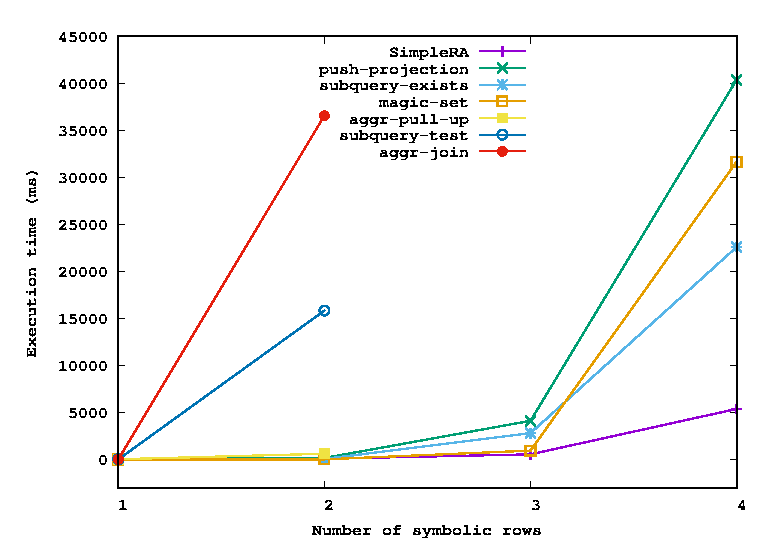
\includegraphics[width=0.7\linewidth]{scale.eps}
  \caption{Number of Symbolic Rows v. Verification Execution Time}
  \label{fig:scale}
\end{figure}

From the figure, we can see that the scalability of the verifier heavily depends 
on the complexity of the rewriting rules.
For those rewriting rules without table join and subquery, it can scales pretty well.
For rewriting rules with either table join or subquery, the prototype implementation can 
not scale well with the growing of the size of the symbolic schema.
Based on our evaluation, queries with both table join and subquery can not scale to schema with
more than 2 rows.

%%% Local Variables:
%%% mode: latex
%%% TeX-master: "writeup"
%%% End:


\bibliographystyle{plain}
\bibliography{writeup}

\end{document}

%%% Local Variables:
%%% mode: latex
%%% TeX-master: t
%%% End:
